\documentclass[10pt,twocolumn,letterpaper]{article}

%% Language and font encodings
\usepackage[english]{babel}
\usepackage[utf8x]{inputenc}
\usepackage[T1]{fontenc}

% xcolor is the package between braces and between brackets is the option that we want to use
\usepackage{fancyhdr}
\usepackage{biblatex}
\usepackage[color]{showkeys}
\usepackage{etoolbox}
\usepackage{graphicx,tabularx}
\usepackage{amsfonts} 

%% Sets page size and margins
\usepackage[a4paper,top=3cm,bottom=2cm,left=3cm,right=3cm,marginparwidth=1.75cm]{geometry}

%% Useful packages
\usepackage{amsmath}
\usepackage[colorlinks=true, allcolors=blue]{hyperref}

\fancypagestyle{plain}{%
  \fancyhead{}
  \fancyfoot{}
  \fancyfoot[R]{\thepage}
  \fancyfoot[L]{[INFOMR] Multimedia Retrieval - Utrecht University}
}
\pagestyle{plain}

\title{%
  3D Mesh Retrieval System \\
  \large Multimedia Retrieval \\
    Utrecht University}
    
\author{
  Fabien Da Costa Barros [0720823]\\
  \url{f.n.dacostabarros@uu.students.nl}
  \and
  LastName2, FirstName2\\
  \url{first2.last2@xxxxx.com}
}

\date{\today}
\addbibresource{refs.bib}                                                                     
\begin{document}

\maketitle

\selectlanguage{english}

\section*{Introduction}

The objective of this project is to choose, parametrise and put in practise of different procedure and algorithms to build a end-to-end MR System. More precisely the focus will be put on 3D mesh retrieval system. From one mesh we have to retrieve all (at least a decent proportion) of similar mesh. The main challenges will be to analyse different features of a 3D mesh. The main steps of the assignments will be to read and display a 3D mesh; then we have to fix and normalise all the 3D meshes in our database. After that we will extract the feature of the meshes to get the essence of what can define the object is in real life to compare this and retrieve similar mesh. At the end we have to improve it so that it can work faster. All of the code can be find on this \href{https://github.com/FDaCostaB/3DMeshRetrievalSystem}{GitHub page}  

\section{Selection and setup the work environment}

We really want to work with Python as both of us as already a good experience and is efficient using it. It is in general easy to set up a new project and install python library and this was one of the main reason of choosing Python for our project. The research of 3D Mesh analysis and visualisation tool as been narrowed to Python libraries. \\ \\
We have discussed the use of PyMesh, PyMeshLab, TriMesh, Open3D, Vedo. To get a nice taste of what each of them can offer we dig in the documentation to compare the differents features. We also complete the step 1 with each of those library to be able to choose after setting up and working (a little) bit with them. \\ \\
	We wanted to be able to open PLY, OFF, OBJ and STL format. PLY and OFF format are discuss in the lecture and OBJ and STL are really common and was the format of the mesh in a version of PRICETON (3D Mesh) database that we found (after having some trouble access the original one). All of them were able to open PLY, OFF, OBJ and STL format so that was not really discriminating. \\ \\
	We try to compare the different re-meshing, repairing and extraction features with our current knowledge and thought that PyMeshLab and Open3D seems to be quite good. Vedo was excluded from the choice at this point as we didn't find enough informations in the documentation even if it looks fancy. Taking into account the short description made on the assignment page of the course's website consolidated our choices as we want something powerful and reliable. The complexity was also one of our requirements as from previous experience less complex library offers less options. \\ \\
	After achieving step 1 with four of those libraries (vedo was exluded) we try to find a balance between number of dependencies, options proposed for visualisation and analysis. We then decide to go with PyMeshLab\cite{pymeshlab} for analyse purposes and Polyscope\cite{polyscope} for visualisation. Polyscope in the visualisation library already used in som PyMeshlab functions as it is not already built-in PyMeshLab. \\ \\
	
\section{Step 1}

	For this step, we have done several tries with PyMesh, PyMeshLab, TriMesh and Open3D to get in touch with the different tools. We get some trouble to set up PyMesh as we have no previous knowledge on docker. That was one of the main issue that we encounter, thanks to this we are thinking to dockerise our application for the assignment so that it can be easier to run on different OS and avoid installing all the dependencies to run it. For the other libraries it was really easy to set up and we mainly wopy-paste the code snippet of the 'Getting started' page of the corresponding library.  Later on  we will only discuss the PymeshLab project. \\ \\
	Our project have three main dependencies : PyMeshLab, Polyscope and Numpy and run with Python 3.9. At the moment, we have two scripts : main.py and render.py. To have a nice overview and organisation of  the project we will try to split as much as possible the different functionalities (mainly different steps) of the project. 'main.py' just verify the number of arguments and call the function render from 'render.py' with the first arguments passed through. This arguments is the name of the file. We prefer to pass it through the command line so that's it make easy to check tens of mesh and quickly inspect if all is working well. \\ \\
	In 'render.py' there is only one function render() : this function load the mesh and call the polyscope function to add the cloud point and the mesh to scene before displaying it. PyMeshLab have a built-in function .show\_polyscope that show a mesh but working around with polyscope with find it more interesting to implement it with the polyscope function to have more control if with to update later. You see the result of the mesh visualisation script at Figure \ref{fig:ant-mesh}. We are happy of the result of the first step. The 3D mesh visualisation windows was one that we preferred among all of the other libraries tested. It have a lot of function and a button to screenshot that make it easier to make the report.


\begin{figure}
\begin{center}
  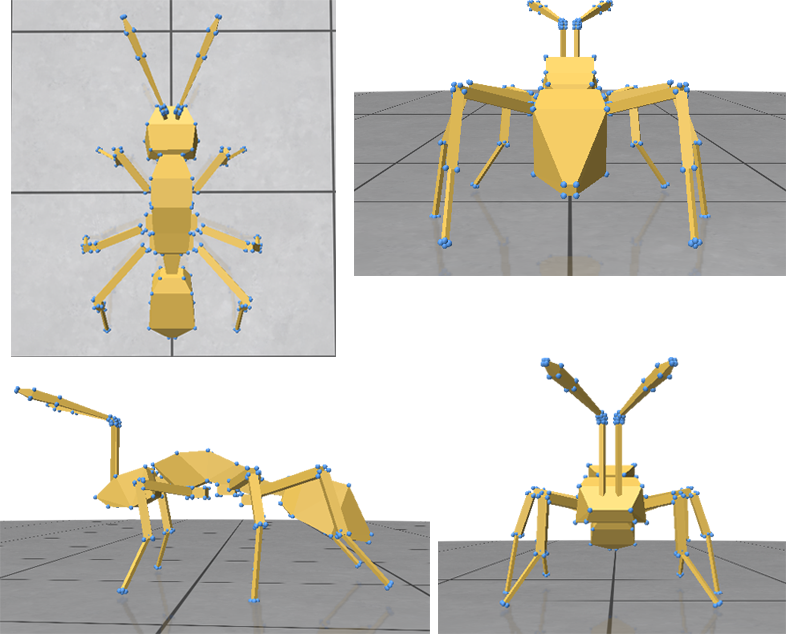
\includegraphics[width=0.5\textwidth]{ant}
  \caption{Visualisation of an ant mesh}
  \label{fig:ant-mesh}
  \end{center}
\end{figure}

%\section*{Acknowledgements}
%Anyone to thank/credit for helping your team along the way? This is the place to do it.

\medskip

\printbibliography

\end{document}
